\documentclass[landscape,a0paper,fontscale=0.292]{baposter}

\usepackage[vlined]{algorithm2e}
\usepackage{times}
\usepackage{calc}
\usepackage{url}
\usepackage{graphicx}
\usepackage{amsmath}
\usepackage{amssymb}
\usepackage{relsize}
\usepackage{multirow}
\usepackage{booktabs}
\usepackage{cancel}
\usepackage{soul}
\usepackage[export]{adjustbox}

\usepackage{graphicx}
\usepackage{multicol}
\usepackage[T1]{fontenc}
\usepackage{ae}
\usepackage{epstopdf}
\usepackage[labelformat=empty,margin={1cm,1cm}]{caption}
\usepackage{wrapfig}


\graphicspath{{images/}}

 %%%%%%%%%%%%%%%%%%%%%%%%%%%%%%%%%%%%%%%%%%%%%%%%%%%%%%%%%%%%%%%%%%%%%%%%%%%%%%%%
 %%%% Some math symbols used in the text
 %%%%%%%%%%%%%%%%%%%%%%%%%%%%%%%%%%%%%%%%%%%%%%%%%%%%%%%%%%%%%%%%%%%%%%%%%%%%%%%%
 % Format 
 \newcommand{\RotUP}[1]{\begin{sideways}#1\end{sideways}}


 %%%%%%%%%%%%%%%%%%%%%%%%%%%%%%%%%%%%%%%%%%%%%%%%%%%%%%%%%%%%%%%%%%%%%%%%%%%%%%%%
 % Multicol Settings
 %%%%%%%%%%%%%%%%%%%%%%%%%%%%%%%%%%%%%%%%%%%%%%%%%%%%%%%%%%%%%%%%%%%%%%%%%%%%%%%%
 \setlength{\columnsep}{0.7em}
 \setlength{\columnseprule}{0mm}


 %%%%%%%%%%%%%%%%%%%%%%%%%%%%%%%%%%%%%%%%%%%%%%%%%%%%%%%%%%%%%%%%%%%%%%%%%%%%%%%%
 % Save space in lists. Use this after the opening of the list
 %%%%%%%%%%%%%%%%%%%%%%%%%%%%%%%%%%%%%%%%%%%%%%%%%%%%%%%%%%%%%%%%%%%%%%%%%%%%%%%%
 \newcommand{\compresslist}{%
 \setlength{\itemsep}{1pt}%
 \setlength{\parskip}{0pt}%
 \setlength{\parsep}{0pt}%
 }


 %%%%%%%%%%%%%%%%%%%%%%%%%%%%%%%%%%%%%%%%%%%%%%%%%%%%%%%%%%%%%%%%%%%%%%%%%%%%%%
 % Formating
 \newcommand{\Matrix}[1]{\begin{bmatrix} #1 \end{bmatrix}}
 \newcommand{\Vector}[1]{\begin{pmatrix} #1 \end{pmatrix}}

 \newcommand*{\norm}[1]{\mathopen\| #1 \mathclose\|}% use instead of $\|x\|$
 \newcommand*{\abs}[1]{\mathopen| #1 \mathclose|}% use instead of $\|x\|$
 \newcommand*{\normLR}[1]{\left\| #1 \right\|}% use instead of $\|x\|$

 \newcommand*{\SET}[1]  {\ensuremath{\mathcal{#1}}}
 \newcommand*{\FUN}[1]  {\ensuremath{\mathcal{#1}}}
 \newcommand*{\MAT}[1]  {\ensuremath{\boldsymbol{#1}}}
 \newcommand*{\VEC}[1]  {\ensuremath{\boldsymbol{#1}}}
 \newcommand*{\CONST}[1]{\ensuremath{\mathit{#1}}}

 \DeclareMathOperator*{\argmax}{arg\,max}
 \DeclareMathOperator*{\diag}{diag}
 \DeclareMathOperator*{\argmin}{arg\,min}
 \DeclareMathOperator*{\vectorize}{vec}
 \DeclareMathOperator*{\reshape}{reshape}

 %-----------------------------------------------------------------------------
 % Differentiation
 \newcommand*{\Nabla}[1]{\nabla_{\!#1}}

 \renewcommand*{\d}{\mathrm{d}}
 \newcommand*{\dd}{\partial}

 \newcommand*{\At}[2]{\ensuremath{\left.#1\right|_{#2}}}
 \newcommand*{\AtZero}[1]{\At{#1}{\pp=\VEC 0}}

 \newcommand*{\diffp}[2]{\ensuremath{\frac{\dd #1}{\dd #2}}}
 \newcommand*{\diffpp}[3]{\ensuremath{\frac{\dd^2 #1}{\dd #2 \dd #3}}}
 \newcommand*{\diffppp}[4]{\ensuremath{\frac{\dd^3 #1}{\dd #2 \dd #3 \dd #4}}}
 \newcommand*{\difff}[2]{\ensuremath{\frac{\d #1}{\d #2}}}
 \newcommand*{\diffff}[3]{\ensuremath{\frac{\d^2 #1}{\d #2 \d #3}}}
 \newcommand*{\difffp}[3]{\ensuremath{\frac{\dd\d #1}{\d #2 \dd #3}}}
 \newcommand*{\difffpp}[4]{\ensuremath{\frac{\dd^2\d #1}{\d #2 \dd #3 \dd #4}}}

 \newcommand*{\diffpAtZero}[2]{\ensuremath{\AtZero{\diffp{#1}{#2}}}}
 \newcommand*{\diffppAtZero}[3]{\ensuremath{\AtZero{\diffpp{#1}{#2}{#3}}}}
 \newcommand*{\difffAt}[3]{\ensuremath{\At{\difff{#1}{#2}}{#3}}}
 \newcommand*{\difffAtZero}[2]{\ensuremath{\AtZero{\difff{#1}{#2}}}}
 \newcommand*{\difffpAtZero}[3]{\ensuremath{\AtZero{\difffp{#1}{#2}{#3}}}}
 \newcommand*{\difffppAtZero}[4]{\ensuremath{\AtZero{\difffpp{#1}{#2}{#3}{#4}}}}

 %-----------------------------------------------------------------------------
 % Defined
 % How should the defined operator look like (:= or ^= ==)
 % (I want back my :=, it is so much better than ^= because (1) it has a
 % direction and (2) everyone here uses it.)
 %
 % Use :=
 %\newcommand*{\defined}{\ensuremath{\mathrel{\mathop{:}}=}}
 %\newcommand*{\definedRight}{\ensuremath{=\mathrel{\mathop{:}}}}
 % Use ^=
 \newcommand*{\defined}{\ensuremath{\triangleq}}
 \newcommand*{\definedRight}{\ensuremath{\triangleq}}
 % Use = with three bars
 %\newcommand*{\defined}{\ensuremath{?}}
 %\newcommand*{\definedRight}{\ensuremath{?}}

 %%%%%%%%%%%%%%%%%%%%%%%%%%%%%%%%%%%%%%%%%%%%%%%%%%%%%%%%%%%%%%%%%%%%%%%%%%%%%%
 % Symbols used in the paper

 %-----------------------------------------------------------------------------
 % The Methods
 \newcommand*{\ICIA}{\emph{ICIA}}
 \newcommand*{\CoDe}{\emph{CoDe}}
 \newcommand*{\LinCoDe}{\emph{LinCoDe}}
 \newcommand*{\CoNe}{\emph{CoNe}}
 \newcommand*{\CoLiNe}{\emph{CoLiNe}}
 \newcommand*{\LinCoLiNe}{\emph{LinCoLiNe}}

 % inter eye distance
 \newcommand*{\ied}{IED}

 %-----------------------------------------------------------------------------
 % Koerper
 %%\newcommand*{\RR}{\mathbb{R}}
 %\newcommand*{\RR}{{I\hspace{-3.5pt}R}}
 %\newcommand*{\RR}{{\mathrm{I\hspace{-2.7pt}R}}}

 \font\dsfnt=dsrom12

 \DeclareSymbolFont{nark}{U}{dsrom}{m}{n}
 \DeclareMathSymbol{\NN}{\dsfnt}{nark}{`N}
 \DeclareMathSymbol{\RR}{\dsfnt}{nark}{`R}
 \DeclareMathSymbol{\ZZ}{\dsfnt}{nark}{`Z}

 %-----------------------------------------------------------------------------
 % Domains
 \newcommand*{\D}{\mathcal{D}}
 \newcommand*{\I}{\mathcal{I}}

 %-----------------------------------------------------------------------------
 % Texture coordinates
 \newcommand*{\rr}{\VEC{r}}

 %-----------------------------------------------------------------------------
 % Parameters
 \newcommand*{\pt}{\VEC{\tau}}
 \newcommand*{\pr}{\VEC{\rho}}
 \newcommand*{\pp}{\VEC{p}}
 \newcommand*{\qq}{\VEC{q}}
 \newcommand*{\xx}{\VEC{x}}
 \newcommand*{\deltaq}{\Delta \qq}
 \newcommand*{\deltap}{\Delta \pp}
 \newcommand*{\zz}{\VEC{z}}
 \newcommand*{\pa}{\VEC{\alpha}}
 \newcommand*{\qa}{\VEC{\alpha}}
 \newcommand*{\pb}{\VEC{\beta}}

 %-----------------------------------------------------------------------------
 % Optimal appearance parameters
 \newcommand*{\pbh}[1]{\ensuremath{\hat{\pb}({#1})}}

 %-----------------------------------------------------------------------------
 % Warp basis
 \newcommand*{\M}[1]{\ensuremath{M({#1})}}
 \newcommand*{\LL}[1]{\ensuremath{L({#1})}}

 %-----------------------------------------------------------------------------
 % Matrices of the texture model
 \newcommand*{\AM}[1]{\ensuremath{\Lambda(#1)}}               % Lambda(beta) 
 \newcommand*{\AMr}[2]{\ensuremath{\Lambda(#1; #2)}}        % Lambda(r, beta)

 \newcommand*{\As}{A}         % Continuous Basis symbol
 \newcommand*{\afs}{a}        % Continuous mean symbol
 \newcommand*{\A}[1]{\As(#1)}         % Continuous Basis
 \newcommand*{\af}[1]{\afs(#1)}        % Continuous mean


 %-----------------------------------------------------------------------------
 % Matrices of the shape model
 \newcommand*{\MU}{\VEC{\mu}}
 \newcommand*{\MM}{\MAT{M}}

 %-----------------------------------------------------------------------------
 %% The project out matrix and operator
 \newcommand*{\INT}{\MAT{P}}
 \newcommand*{\INTf}{P}

 %-----------------------------------------------------------------------------
 % The identity matrix
 \newcommand*{\EYEtwo}{\Matrix{1 & 0\\0&1}}
 \newcommand*{\EYE}{\MAT E}
 \newcommand*{\EYEf}{E}

 % Wether to use subscripts or brackets for some function arguments
 % can be decided by commenting out the corresponding functions underneath
 %-----------------------------------------------------------------------------
 % Mapping
 \newcommand*{\Cs}[1]{\ensuremath{C^{#1}}} % C symbol
 \newcommand*{\C}[2]{\ensuremath{C^{#1}(#2)}} % Use C with brackets

 %-----------------------------------------------------------------------------
 % Objective function
 \newcommand*{\Fs}{\ensuremath{F}}              % F symbol
 \newcommand*{\F}[1]{\ensuremath{\Fs(#1)}}       % Use F with brackets    F(q)

 %-----------------------------------------------------------------------------
 % Approximated objective functions
 \newcommand*{\FFs}{\tilde{F}}                     % ~F symbol
 \newcommand*{\FF}[1]{\ensuremath{\FFs(#1)}}       % Use ~F with brackets    F(q)

 %-----------------------------------------------------------------------------
 % residual function
 \newcommand*{\es}{\ensuremath{f}}              % R symbol

 \newcommand*{\e}[1]{\ensuremath{\es(#1)}}         % R(q)
 \newcommand*{\er}[2]{\ensuremath{\es(#1; #2)}}    % R(r; q)

 %-----------------------------------------------------------------------------
 % Approximated residual functions
 \newcommand*{\ees}{\tilde{f}}                       % ~R symbol
 \newcommand*{\ee}[1]{\ensuremath{\ees(#1)}}       % ~R(q)
 \newcommand*{\eer}[2]{\ensuremath{\ees(#2; #1)}}  % ~R(r; q)

 %-----------------------------------------------------------------------------
 % Warps
 \newcommand*{\Vs}{\ensuremath{V}}
 \newcommand*{\VLins}{\ensuremath{\Vs^{\text{Ortho}}}}
 \newcommand{\VModels}{\ensuremath{\Vs^{\text{Model}}}}
 \newcommand*{\Ws}{\ensuremath{W}}

 \newcommand{\V}[1]{\ensuremath{\Vs(#1)}}
 \newcommand{\VModel}[1]{\ensuremath{\VModels(#1)}}
 \newcommand{\Vr}[2]{\ensuremath{\Vs(#1; #2)}}
 \newcommand{\VInvr}[2]{\ensuremath{\Vs^{-1}(#1; #2)}}
 \newcommand{\VrLin}[2]{\ensuremath{\VLins(#1; #2)}}
 \newcommand{\W}[1]{\ensuremath{\Ws(#1)}}
 \newcommand{\Winv}[1]{\ensuremath{\Ws^{-1}(#1)}}
 \newcommand{\Wr}[2]{\ensuremath{\Ws(#1; #2)}}


%%%%%%%%%%%%%%%%%%%%%%%%%%%%%%%%%%%%%%%%%%%%%%%%%%%%%%%%%%%%%%%%%%%%%%%%%%%%%
%% Begin of Document
%%%%%%%%%%%%%%%%%%%%%%%%%%%%%%%%%%%%%%%%%%%%%%%%%%%%%%%%%%%%%%%%%%%%%%%%%%%%%
\begin{document}
%%%%%%%%%%%%%%%%%%%%%%%%%%%%%%%%%%%%%%%%%%%%%%%%%%%%%%%%%%%%%%%%%%%%%%%%%%%%%
%% Here starts the poster
%%---------------------------------------------------------------------------
%% Format it to your taste with the options
%%%%%%%%%%%%%%%%%%%%%%%%%%%%%%%%%%%%%%%%%%%%%%%%%%%%%%%%%%%%%%%%%%%%%%%%%%%%%
\begin{poster}{
 % Show grid to help with alignment
 grid=false,
 % Column spacing
 colspacing=0.7em,
 % Color style
 headerColorOne=cyan!20!white!90!black,
 borderColor=cyan!30!white!90!black,
 % Format of textbox
 textborder=faded,
 % Format of text header
 headerborder=open,
 headershape=roundedright,
 headershade=plain,
 background=none,
 bgColorOne=cyan!10!white,
 headerheight=0.12\textheight}
 % Eye Catcher
{
  \begin{tabular}{l}
    
\includegraphics[height=0.1\textheight]{odulogo.eps}
  \end{tabular}
 } 
 % Title
 {\sc{\vspace{0.1em} \Huge Making Enterprise-Level Archive Tools}\\Accessible for Personal Web Archiving} 
 % Authors
 {\vspace{-0.3em}Mat Kelly, Michele C. Weigle, and Michael L. Nelson\\
 {\vspace{-0.3em}\texttt{\{mkelly,mweigle, mln\}@cs.odu.edu}}\\
 Department of Computer Science, Old Dominion University, Norfolk, Virginia USA}
 % University logo
 {
  \begin{tabular}{r}
    
\includegraphics[height=0.1\textheight]{odulogo.eps}
  \end{tabular}
 }

  \headerbox{One-Click, User Instigated Preservation}{name=flow,column=0,row=0,span=4}{
  \centering 	
\begin{minipage}[c]{11.0cm}
\centering
	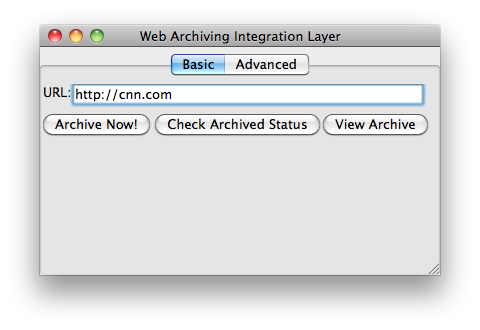
\includegraphics[height=8.0cm]{cnn_wail.png}
  \captionof{figure}[One figure]{$\bullet$\ \ ``Archive Now!'' button sets up crawl, initiates crawl and puts archive file in correct location to be indexed.\\
  $\bullet$\ \ Wayback consumption can be checked with ``Check Archive Status'' button. }
  \label{medium}
\end{minipage}
\hspace{0.0cm}
\begin{minipage}[c]{11.0cm}
\centering
	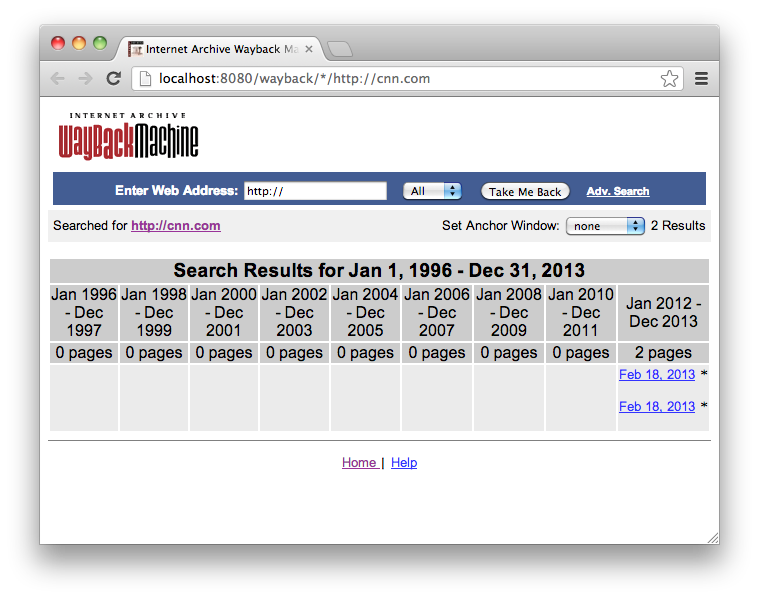
\includegraphics[height=8.0cm]{cnn_wayback.png}
	  \captionof{figure}[One figure]{$\bullet$\ \ Once indexed, ``View Archive'' button shows all archives for URL in local Wayback.}
  \label{medium}
\end{minipage}
\hspace{0.0cm}
\begin{minipage}[c]{11.0cm}
\centering
	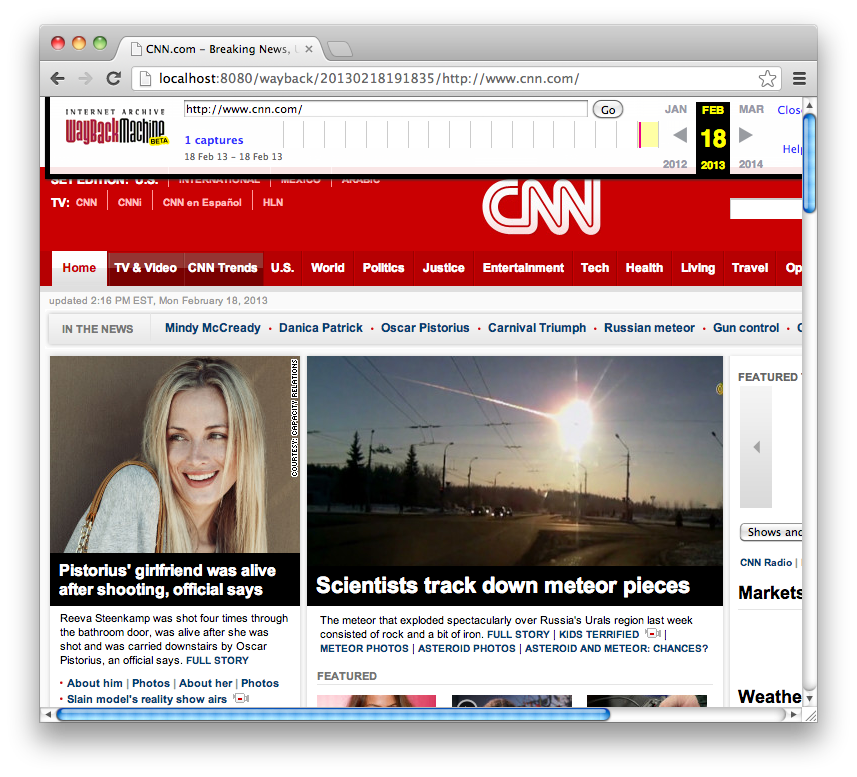
\includegraphics[height=8.0cm]{cnn_replay.png}
	  \captionof{figure}[One figure]{$\bullet$\ \ Selecting the date in local Wayback displays the preserved webpage.}
  \label{medium}
\end{minipage}

  }

\headerbox{Features}{name=features,column=0,row=0,span=1,below=flow}{
  
\begin{itemize}
\item Collection of Archiving Tools
\item Drag \& Drop Installation And Removal
\item All Tools Can Reside on a Single Machine
\item Managed Through a Graphical User Interface (GUI)
\end{itemize}

}

\headerbox{Tools Installed Locally}{name=guicontrol,column=1,row=0,span=1,below=flow}{
  
\begin{itemize}
\item \textbf{CREATE ARCHIVES:} Heritrix (Crawler) 
\item \textbf{REPLAY ARCHIVES:} Wayback Machine
\item \textbf{INSPECT ARCHIVES:} WARC-Proxy
\item More to Come!
\end{itemize}

}

  
  





 %\headerbox{How the Tools Fit Together}{name=toolHierarchy,column=0,row=0,span=2,below=features}{
 %	\centering
 %	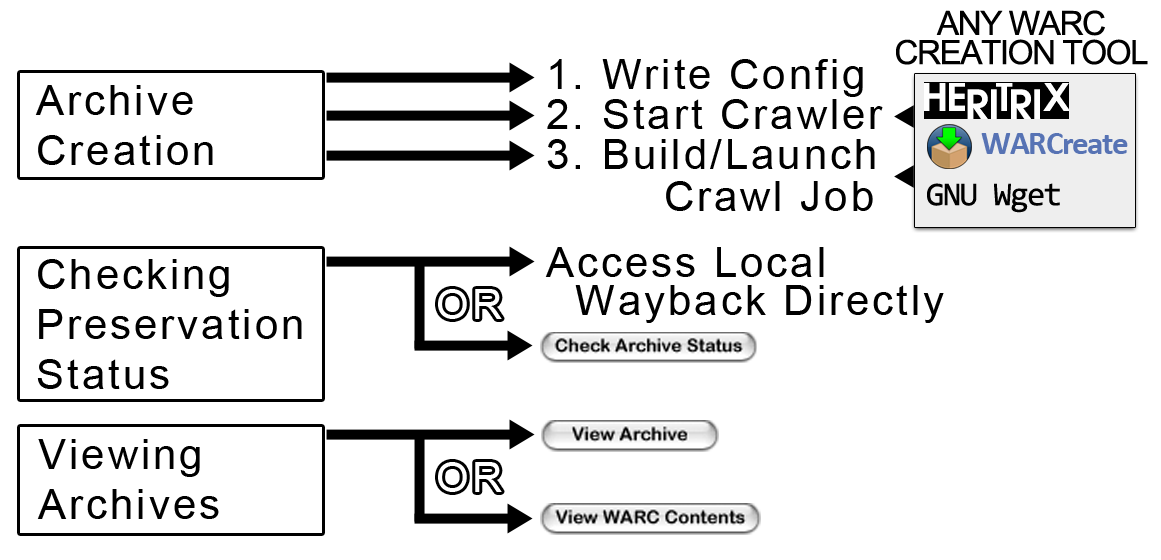
\includegraphics[height=5.5cm]{process.png}
 %}

%\headerbox{A Sample Archiving Session}{name=samplearchiving,column=2,span=2,below=toolHierarchy}{
%	\begin{tabular}{p{7.5cm} |p{7.5cm}}
%	    \textbf{\underline{Creating Archives (Simple)}} & \textbf{\underline{Creating Archives (Custom)}} \\
%		1. Input URL 					& 1. Hit ``Start Heritrix Process'' Button	  \\
%		2. Hit ``Archive Now'' Button 	& 2. Input List of URLs \\
%		         						& 3. Hit ``Write Heritrix Config'' Button \\
%		         						& 4. (Optionally) Customize Crawl Job XML in Heritrix Interface (or local file)\\
%		         						& 5. Hit ``Launch Crawl'' Button
%	\end{tabular}
%	
%}

\headerbox{Advanced Options/Features}{name=advanced,column=0,row=0,span=2,below=features}{
	\begin{itemize}
		\item Specify Multiple URLs to be Included in the Crawl
		\item Setup Crawls and Allow for Customization Prior to Execution (e.g., crawl period)
		\item Start or Stop Services Not Currently Needed (e.g., initialize a long crawl but delay replay until later)
	\end{itemize}	
	
}

 \headerbox{Interface for Tweaking}{name=screenshot,column=2,row=0,span=1,below=flow}{
 	\centering
 	%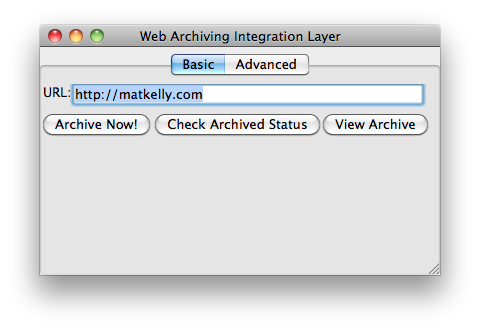
\includegraphics[scale=0.45,keepaspectratio,valign=t,margin=0cm 0cm]{wail_basic.png}
    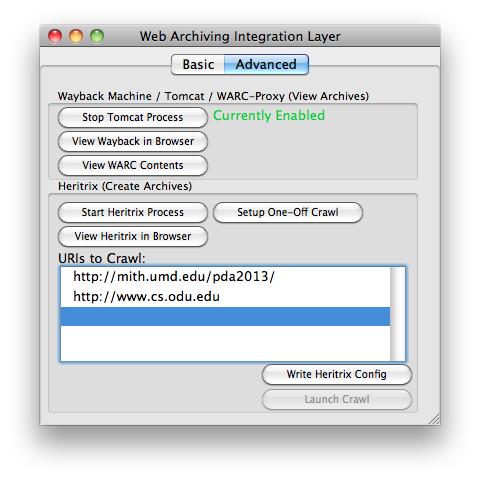
\includegraphics[scale=0.4,keepaspectratio,valign=t,margin=0cm 0cm]{wail_advanced.png} 	
 }

\headerbox{Support}{name=misc,column=3,row=0,span=1,below=flow}{
 	\begin{itemize}
 		\item \textbf{GENERATED ARCHIVES ARE SAFE}\\Web ARChives (WARCs) reside on your hard drive, can be backed up for safe keeping like any other file
 		\item \textbf{CROSS PLATFORM}\\Support for MacOS X, Windows and Linux
 		\item \textbf{WORKS WITH EXISTING WARCS}\\Just drop in and local Wayback will index for replay
 		\item \textbf{COMPATIBLE WITH OTHER ARCHIVING TOOLS}\\Use the WARC-generating preservation tool of your choice (e.g., WARCreate, Wget) in lieu of Heritrix
 	\end{itemize}
 }


% \headerbox{NOT YET INCLUDED IN POSTER}{name=notYetIncluded,column=2,row=0,span=2,below=samplearchiving}{
%	\begin{itemize}
%		\item WARCs are portable, you are not locked into the tool
%		\item Win7, OS X and Linux compatibility
%		\item Explanation of why XAMPP is not needed (only Tomcat)
%		\item Any descriptors of the GUI. Are these necessary? Are ``pics worth 1000 words''?
%	\end{itemize}	 
% 
% }


 %%%%%%%%%%%%%%%%%%%%%%%%%%%%%%%%%%%%%%%%%%%%%%%%%%%%%%%%%%%%%%%%%%%%%%%%%%%%%%
%   \headerbox{References}{name=references,column=0,above=bottom,below=bigdiagram,span=2}{
% 
% %%%%%%%%%%%%%%%%%%%%%%%%%%%%%%%%%%%%%%%%%%%%%%%%%%%%%%%%%%%%%%%%%%%%%%%%%%%%%%
%     \smaller
%     
%     \bibliographystyle{ieee}
%     \renewcommand{\section}[2]{\vskip 0.05em}
%       \begin{thebibliography}{1}\itemsep=-0.01em
%       \setlength{\baselineskip}{0.4em}
%	
%       \bibitem{bergman}
%       M. K. ~Bergman
%       \newblock The deep web: Surfacing the hidden value.
%       \newblock {\em Journal of Electronic Publishing}, 2000.
%
%		\bibitem{iso}
%		ISO.
%		\newblock Information and documentation - WARC file format, 2009
%		
%		\bibitem{Marshall_2008}
%		C. C. ~Marshall
%		\newblock Rethinking Personal Digital Archiving, Part 1: Four Challenges from the Field.
%		\newblock {\em D-Lib Magazine}, 14(3/4):2, 2008.
%
%		\bibitem{Marshall_2006}
%		C. C. ~Marshall, S. A. ~Bly, and F. ~Brun-Cottan
%		\newblock The Long Term Fate of Our Digital Belongings: Toward a Service Model for Personal Archive
%		\newblock In {\em Proceedings of IS\& T Archiving}, pages 25-30, 2006.
%		
%		\bibitem{Marshall_2007}
%		C. C. ~Marshall, F. ~McCown, and M. L. ~Nelson
%		\newblock Evaluating Personal Archiving Strategies For Internet-Based Information
%		\newblock In {\em Proceedings of IS\& T Archiving}, pages 151-156, 2007.		
%		
%		\begin{center}
%		{\normalsize JCDL 2012; Washington, DC; June 11, 2012}
%		\end{center}
%       \end{thebibliography}
%   }

 %\headerbox{}{name=urls,column=0,below=futureWork,span=4}{
 %	\begin{multicols}{3}{
 %	JCDL 2012; Washington, DC; June 11, 2012\\
 %	\\
 %	\url{http://ws-dl.blogspot.com/}
 %	}
 %	\end{multicols}
 %} 


\headerbox{}{name=confName,column=0,span=2,below=screenshot,headerColorOne=white,headerborder=none,textborder=bars,borderColor=white}{
\begin{center}\Large
PDA 2013; College Park, MD; February 21, 2013
\end{center}
}

\headerbox{}{name=screenshot,column=2,span=2,below=screenshot,headerColorOne=white,headerborder=none,textborder=bars,borderColor=white}{
\begin{center}\Large
http://matkelly.com/wail
\end{center}
}

\end{poster}%
%
\end{document}
